\chapter{Introduction}


\section{A Problem}
Consider an image of a face. At least two \emph{systems} are at play in the image of a face, the face itself and the illumination. Both face and illumination are complex and can vary greatly, but they are fundamentally acting independently of each other up until they compose to form the image.

A form of Deep Neural Networks, Deep Belief Networks, have achieved state of the art performance in facial recognition, but this is only possible with a large amount of training data. This suggests that there is a disparity between the task and these networks, as the networks do no explicitly attempt to represent these \emph{systems} indedependently. This project takes steps toward representing complex causes separately with the primary task of decomposing joint images (more generally, vector based data).

Separating faces and illumination is too challenging for this project, there is no way to verify/evaluate that the new approach is working as the concept of a face without illumination cannot be visualised. Instead I will start with the modest task of working with images where the source images being combined are known.

\section{Deep Belief Networks can achieve state of the art performance}
Deep Belief networks (DBNs) are powerful models that have proven to achieve state of the art performance in tasks such as image classification, dimensionality reduction, natural language recognition, Document classification, Semantic Analysis.\todocite{}
Despite a DBN's expressiveness, there is no way to extract independant sources, the model instead learns how to represent the complex combination. The complex combination of sources is inheriently richer than the individual sources acting alone. The DBN may learn features that correspond to each source during it's training process, however the architecture or training algorithm make no attempt to enforce this. Consider face and illumination example, with 1000 possible faces and 1000 possible illuminations. If we only observe a combination of faces and illuminations there is 1000000 possible combinations we need to represent. It is more succint to treat faces and illuimination as independent \emph{system}, resulting in 2000 combinations.

DBNs are built of shallow networks called Restricted Boltzmann Machines (RBMs). Despite being building blocks for the DBN RBMs can be used as models for practical tasks for instance representing handrwritten digits \cite{fischer2014training}.

\section{A Proposed Solution and Contributions}

Frean and Marsland propose an alternative architecture to that of an RBM, that aims to encode two complex sources independantly. Frean and Marsland also propose an algorithm to put this alternative architecture to use.

This project contributes:
\begin{enumerate}[$\mathcal{C}$1.]
  \item\label{item-c1} The first articulation of the proposed architecture, including the context needed to understand it.
  \item\label{item-c2} A Python implementation of the new architecture.
  \item\label{item-c3} A suite of graded evaluations/tests that explore how the architecture and source separation algorithm work in practice.
\end{enumerate}
The evaluations will not address separating faces and illumination, instead only performing tasks such as separating two handwritten digits composed on each other (see figure \ref{F:Composition-Example}).

\begin{figure}[h]
\begin{center}
  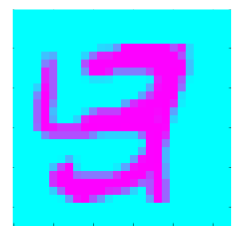
\includegraphics[width = 0.1\textwidth]{Assets/composition-example.png}
\caption{An example composition of a handwritten four and three, illustrating a non-trival task where the ground truth is known.}
\label{F:Composition-Example}
\end{center}
\end{figure}


%
% The shared views of four research groups, including the prolific Geoffrey Hinton, is that DBNs are favoured for use in speech recognition tasks over other deep learning approaches~\cite{Hinton:38131ww}. For instance \texttt{Stacked Denoising Autoencoders} and \texttt{Deep Convolutional Networks}.
%
%
% \subsection{Aspirational Examples as a motivation of the project}
%
% Now some thought experiments to highlight a fundamental weakness in DBNs.
%
% DBNs can capture rich non-linearity, making them ideal for tasks such as facial recognition, where pixels in the images change drastically depending on pose and illumination. These variations impede the use of classical feature based on geometry, such as Eigenfaces or Fischer-face~\cite{Lin:6100469ww}. There are at least two systems at play in an image of a face, the face itself that has a shape and colour, and the illumination which can vary greatly, casting shadows and highlighting parts of the face. Despite this, a DBN can achieve excellent classification performance on the UMIST dataset of 576 multi-viewed faced images of 20 individuals~\cite{Lin:6100469ww}.
%
% Consider another famous example that illustrates the idea of multiple sources acting independently to form some data, referred to as the \texttt{Cocktail Party Problem}. At a cocktail party many conversations are taking part at the same time, yet despite the cacophony, a partygoer is able to take part in their conversation, separating the sources.
%
% Both these examples exhibit independent sources arising and interacting in a non-linear way to generate a visible artifact, be it an image of a face or a audio recording. This project does not address these aspirational examples, they set the scene for it's motivation. Despite a DBN's expressiveness, there is no way to extract these sources, the model instead learning the how to represent the combination. The DBN might fully well learn features that correspond to each source during it's training process, however the architecture or training algorithm make no attempt to enforce this.
%
% % Deep Belief Networks are constructed by stacking Restricted Boltzmann Machines (RBMs). This proved a natural starting point for representing two sources. We worked in a shallow environment before attempting to stack RBMs.
% \subsection{Restricted Boltzmann Machines cannot separate sources either}
%
% DBNs are composed of a models with a shallow architecture, Restricted Boltzmann Machines (RBMs). RBMs provide a natural starting point for representing data causes by the combination of two sources.
%
% RBMs are two layer, fully connected, unsupervised neural networks. RBMs do not model causation, instead they model dependancies.
% % RBMs make a strong assumption that all features are dependant in the prior, inheriently modelling a single source.
%
%   % In the image domain, this equates to all pixels being assumed relevant to what we are trying to model. With enough examples RBMs can generalise, but there is no mechanism for modelling independant subjects.
%   Again using the example of images, an input image will map to a single representation. There lacks a mechanism for modeling  sources that are acting independantly, instead modeling inputs as a single source.
%
% % There is another structure, Belief/Bayesian Networks, and the parameterised version, the Sigmoid Belief Network, which makes the polar assumption where each feature is modelled by an independant cause. These are intractable to train in practice.
% \subsection{Sigmoid Belief Networks --- Intractably causal in practice}
% The Sigmoid Belief Network, the parameterized version of a Bayesain/Belief network appears as a natural choice for modelling independent sources in that it makes a polar assumption to the RBM; -- Warning Semicolon Use -- Every feature has an independant cause. The sigmoid belief networks assumption could capture data that has multiple sources, but this is intractable in practice.
%
% % Frean, Marsland propose a generative model that aims for a middle ground between these two existing models.
% \section{A proposed solution}
% \subsection{Trading tractibility for Source Separation}
% Frean and Marsland propose a generative model that aims to trade a small amount of the RBMs performance for richness, finding a middle ground between the Sigmoid Belief network and the Restricted Boltzmann Machine.
% Frean and Marsland also propose an algorithm to invert this proposed generative model, seperating the sources of an input.
%
% The new generative model, referred to onwards as an ORBM, uses an RBM to model each source and a sigmoid belief network to capture their combination to from data. This project explores the ORBM use for separating two causes.
%
% \begin{figure}[h]
% \begin{center}
%   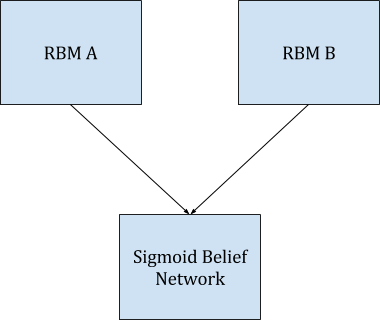
\includegraphics[width = 0.5\textwidth]{Assets/ORBM_fig_1}
% \caption{A graphical representation showing the proposed generative model for capturing two causes, the ORBM.}
%
% \label{F:ORBM-fig-1}
% \end{center}
% \end{figure}
%
% Given the proposed model and algorithm, this project answers the following questions:
% \begin{itemize}
%   \item Can the ORBM represent two sources of composite data independent, that is can it be used to perform source separation?
%   \item Is the ORBMs two cause structure to rich to be tractable in practice?
% \end{itemize}
%
% \section{Results and Contribution}
%
% This project provides a suite of evalautions, in the form of tests of increasing complexity to answer the above questions. The aim being to incrementally verify the new generative model and inference algorithm.
%
% The tests give reasons for optimism, especially in the smaller cases. Challenges have been exposed in the evaluation that will need to be addressed going forward, to make the algorithm and model scalable.
